\documentclass[11pt]{scrartcl}
\usepackage{tikz}
\usetikzlibrary{%
  arrows,
  calc
}

\begin{document}
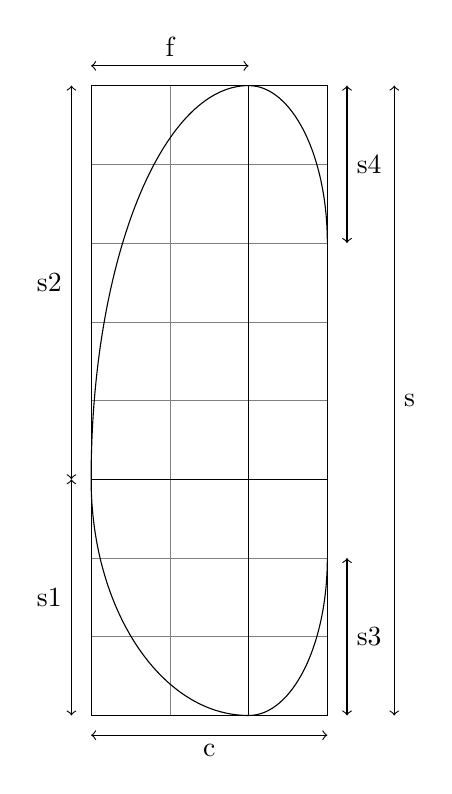
\begin{tikzpicture}

  \draw[help lines] (0,0) grid (3,8);

  \draw (0,0) -- (3,0) -- (3,8) -- (0,8) -- cycle;
  \draw (2,0) -- (2,8);
  \draw (0,3) -- (3,3);

  \draw (2,0) arc [
                start angle=-90,
                end angle = 0,
                x radius = 1,
                y radius = 2];
  \draw (3,6) arc [
                start angle=0,
                end angle = 90,
                x radius = 1,
                y radius = 2];
              \draw (3,2) -- (3,6);
  \draw (2,8) arc [
                start angle=90,
                end angle = 180,
                x radius = 2,
                y radius = 5];
  \draw (0,3) arc [
                start angle=180,
                end angle = 270,
                x radius = 2,
                y radius = 3];
  \draw[<->] (0,-.25) --node[below] {c} (3,-0.250);
  \draw[<->] (-0.25,3) -- node[left] {s2} (-0.25,8);
  \draw[<->] (-0.25,0) -- node[left] {s1} (-0.25,3);
  \draw[<->] (3.25,0) -- node[right] {s3} (3.25,2);
  \draw[<->] (3.25,6) -- node[right] {s4} (3.25,8);
  \draw[<->] (3.85,0) -- node[right] {s} (3.85,8);
  \draw[<->] (0,8.25) -- node[above] {f} (2,8.25);
\end{tikzpicture}
\end{document}
